\documentclass[a4paper,12pt]{article} 
\usepackage[T2A]{fontenc}			
\usepackage[utf8]{inputenc}			
\usepackage[english,russian]{babel}	
\usepackage{amsmath,amsfonts,amssymb,amsthm,mathrsfs,mathtools} 
\usepackage{cancel}
\usepackage{multirow}
\usepackage[colorlinks, linkcolor = blue]{hyperref}
\usepackage{upgreek}\usepackage[left=2cm,right=2cm,top=2cm,bottom=3cm,bindingoffset=0cm]{geometry}
\usepackage{graphicx,wrapfig,subfig}
\usepackage{xcolor}
\graphicspath{ {./images/} }

\author{Толстикова М.С.\\
Группа Б04-205}

\title{\textbf{3.3.4. Эффект Холла в полупроводниках.}}

\date{21 сентября 2023 г.}

\begin{document}
\maketitle

\leftskip=1cm \rightskip=1cm

\textbf{Цель работы}: измерение подвижности и концентрации носителей заряда в полупроводниках.

\textbf{В работе используются}: электромагнит с регулируемым источником питания; вольтметр; амперметр; миллиамперметр; милливеберметр или миллитесламетр; источник питания (1,5 В), образцы легированного германия.

\leftskip=0cm \rightskip=0cm

\section{1. Теоритические сведения.}
Суть эффекта Холла состоит в следующем. Пусть через однородную пластину металла вдоль оси $x$ течет ток $I$ (рис. 1).
	
	\begin{wrapfigure}{l}{0.6\textwidth}
		\vspace{-20pt}
		\begin{center}
		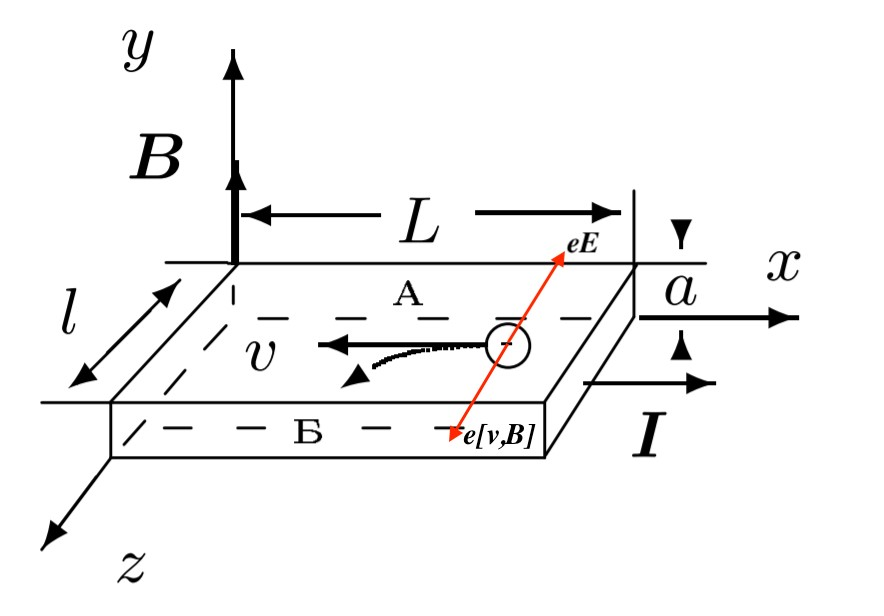
\includegraphics[width=0.7\linewidth]{Holl1.png}
			\label{fig:sdfsafd}
		\end{center}
		\vspace{-20pt}
		\caption{Образец с током в магнитном поле}
	\end{wrapfigure}

	Если эту пластину поместить в магнитное поле, направленное по оси y, то между гранями А и Б появляется разность потенциалов. 
	
	В самом деле, на электрон (для простоты рассматриваем один тип носителей), движущийся со средней скоростью $\langle \vec{v} \rangle$ в электромагнитном поле, действует сила Лоренца:
	
	$$\vec{F}_{л} = -e\vec{E}-e \langle \vec{v} \rangle \times \vec{B},$$
	
	где $e$- абсолютный заряд электрона, $\vec{E}$ - напряженность электрического поля, $\vec{B}$ - индукция магнитного поля.
	
	В проекции на ось $z$ получаем
	
	$$ F_{B}=e | \langle {v_{x}} \rangle | B.$$
	
	Под действием этой силы электроны отклоняются к грани Б, заряжая ее отрицательно. На грани А накапливаются нескомпенсированные положительные заряды. Это приводит к возникновению электрического поля $E_{z}$, направленного от А к Б, которое действует на электроны с силой $F_{E}=eE_{z}$. В установившемся режиме $F_{E}=F_{B}$, поэтому накопление электрических зарядов на боковых гранях пластины прекращается. Отсюда
	
	$$ E_{z}=| \langle {v_{x}} \rangle | B.$$
	
	С этим полем связана разность потенциалов $$U_{AБ}=E_{z}l=| \langle {v_{x}} \rangle | Bl.$$
	
	В этом и состоит эффект Холла.
	
	\
	
	Замечая, что сила тока
	
	$$ I=ne| \langle {v_{x}} \rangle |la,$$
	
	найдем ЭДС Холла:
	
\begin{equation}\label{Rx}
\mathscr{E}_{X}=U_{AБ}=\dfrac{IB}{nea}=R_{X}\dfrac{IB}{a}
\end{equation}
	
	Константа $R_{X}=\dfrac{1}{ne}$ называется постоянной Холла.
	
	В полупроводниках, когда вклад в проводимость обусловлен и электронами и дырками, выражение для постоянной Холла имеет более сложный вид:
	
	$$R_{X}=\dfrac{nb^{2}_{e}-pb^{2}_{p}}{e(nb_{e}+pb_{p})^{2}},$$
	
	где $n$ и $p$ - концентрации электронов и дырок, $b_{e}$ $b_{p}$ - их подвижности.

 \section*{2. Экспериментальная установка.}

	\begin{figure}[h!]
		\centering
		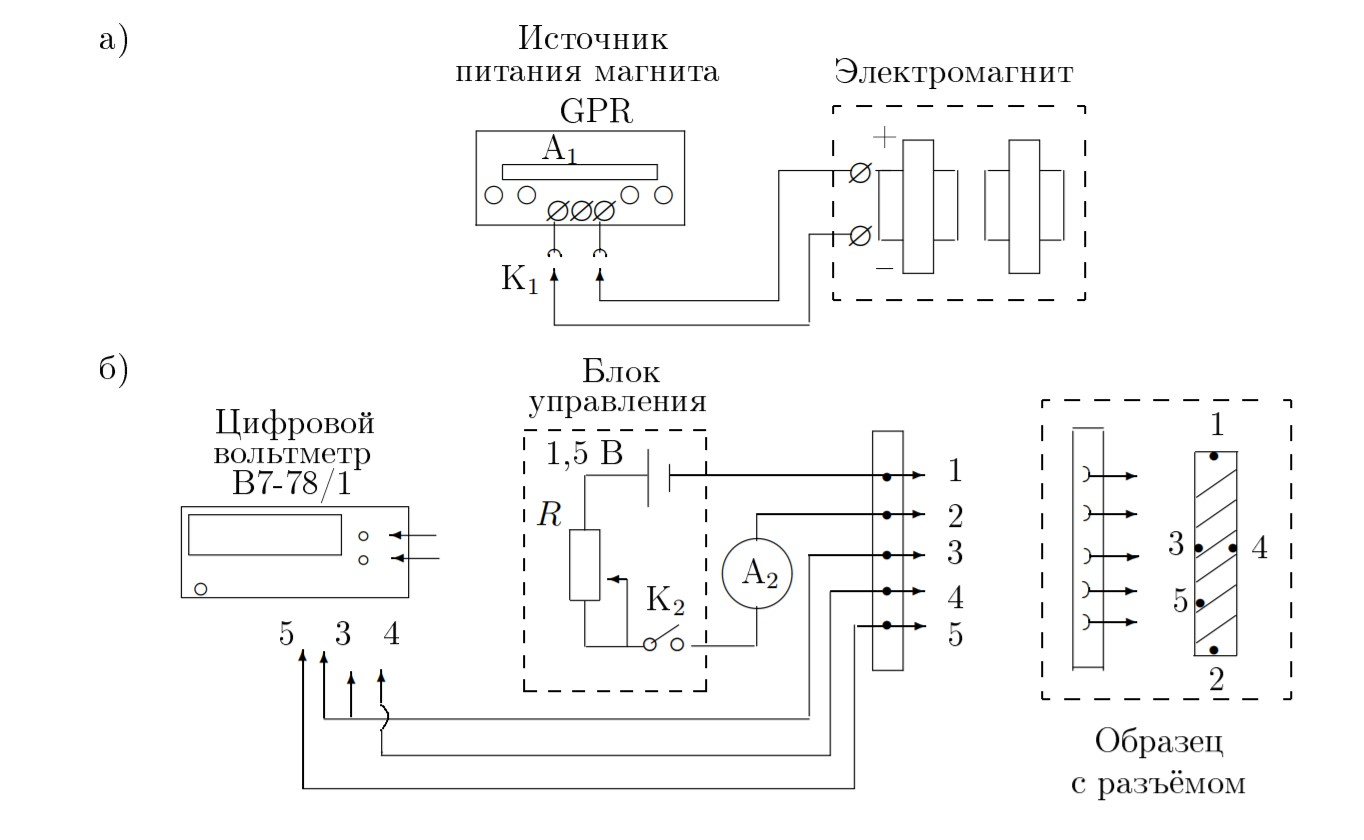
\includegraphics[scale = 0.35]{Holl2}
		\caption{Схема установки для исследования эффекта Холла в полупроводниках}
		\label{fig:Holl2}
	\end{figure}
  
  	В зазоре электромагнита (рис. 2а) создаётся постоянное магнитное поле, величину которого можно менять с помощью регуляторов источника питания. Ток измеряется амперметром источника питания $A_{1}$. Разъем $K_{1}$ позволяет менять направление тока в обмотках электромагнита.
  
  	Образец из легированного германия, смонтированный в специальном держателе (рис. 2б), подключается к батарее. При замыкании ключа $K_{2}$ вдоль длинной стороны образца течет ток, величина которого регулируется реостатом $R$ и измеряется миллиамперметром $A_2$.
  	
  	В образце с током, помещённом в зазор электромагнита, между контактами 3 и 4 возникает разность потенциалов $U_{34}$, которая измеряется с помощью цифрового вольтметра.
  	
  	Контакты 3 и 4 вследствие неточности подпайки не всегда лежат на одной
  	эквипотенциали, и тогда напряжение между ними связано не только с эффектом
  	Холла, но и с омическим падением напряжения, вызванным протеканием основного тока через образец.
  	
  	Измеряемая разность потенциалов при одном направлении
  	магнитного поля равна сумме ЭДС Холла и омического падения напряжения, а
  	при другом  их разности. В этом случае ЭДС Холла $\mathscr{E}_{X}$ может быть определена как половина алгебраической разности показаний вольтметра, полученных для
  	двух противоположных направлений магнитного поля в зазоре.
  	
  	Можно исключить влияние омического падения напряжения иначе, если при каждом токе через образец измерять напряжение между точками 3 и 4 в отсутствие магнитного поля. При фиксированном токе через образец это дополнительное к ЭДС Холла напряжение $U_{0}$ остается неизменным. От него следует (с учетом
  	знака) отсчитывать величину ЭДС Холла: 
  	
  	$$\mathscr{E}_{X} = U_{34} \pm U_{0}$$. 
  	
  	При таком способе измерения нет необходимости проводить повторные измерения с противоположным направлением магнитного поля.
  	
  	
  	По знаку $\mathscr{E}_{X}$ можно определить характер проводимости - электронный или дырочный. Для этого необходимо знать направление тока в образце и направление
  	магнитного поля.
  	
  	Измерив ток $I$ в образце и напряжение $U_{35}$ между контактами 3 и 5 в отсутствие магнитного поля, можно, зная параметры образца, рассчитать проводимость материала образца по формуле:
  	
  \begin{equation}\label{sigma}
  	\sigma=\dfrac{IL_{35}}{U_{35}al}
  \end{equation}
  	
  	где $L_{35}$ - расстояние между контактами 3 и 5, $a$ - толщина образца, $l$ - его ширина.
   
\section*{3. Ход работы.}

$a = 1$ мм; $l_{3,5} = 5$ мм; $l = 4$ мм; $SN = 75$ 

\subsection*{3.1. Расчет индукции магнитного поля.}
\newpage
\begin{figure}[h]
    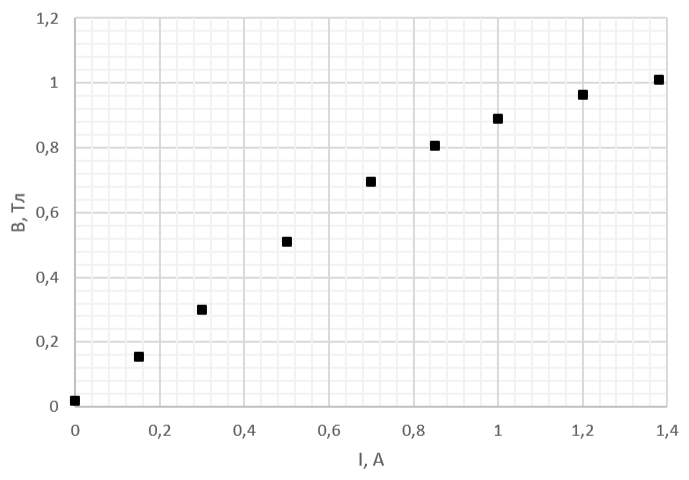
\includegraphics[scale=0.5]{1.png}
    \centering
    \caption*{Калибровочный график электромагнита.}
\end{figure}

\subsection*{3.2. Измерение ЭДС Холла.}

Для разных $ I $ через образец снимем зав-ть ЭДС Холла от тока $ I_\text{м} $ через электромагнит:

\begin{table}[!ht]
\centering
\begin{tabular}{|ll|ll|ll|ll|ll|l}
\cline{1-10}
\multicolumn{2}{|l|}{I = 0,3 mA}      & \multicolumn{2}{l|}{I = 0,4 mA}      & \multicolumn{2}{l|}{I = 0,5 mA}      & \multicolumn{2}{l|}{I = 0,6 mA}      & \multicolumn{2}{l|}{I = 0,7 mA}      &  \\ \cline{1-10}
\multicolumn{1}{|l|}{Im, A} & U34, mV & \multicolumn{1}{l|}{Im, A} & U34, mV & \multicolumn{1}{l|}{Im, A} & U34, mV & \multicolumn{1}{l|}{Im, A} & U34, mV & \multicolumn{1}{l|}{Im, A} & U34, mV &  \\ \cline{1-10}
\multicolumn{1}{|l|}{0}     & 0,004   & \multicolumn{1}{l|}{0}     & 0,005   & \multicolumn{1}{l|}{0}     & 0,005   & \multicolumn{1}{l|}{0}     & 0,007   & \multicolumn{1}{l|}{0}     & 0,007   &  \\ \cline{1-10}
\multicolumn{1}{|l|}{0,15}  & 0,036   & \multicolumn{1}{l|}{0,15}  & 0,047   & \multicolumn{1}{l|}{0,15}  & 0,06    & \multicolumn{1}{l|}{0,15}  & 0,072   & \multicolumn{1}{l|}{0,15}  & 0,089   &  \\ \cline{1-10}
\multicolumn{1}{|l|}{0,3}   & 0,07    & \multicolumn{1}{l|}{0,3}   & 0,093   & \multicolumn{1}{l|}{0,3}   & 0,116   & \multicolumn{1}{l|}{0,3}   & 0,14    & \multicolumn{1}{l|}{0,3}   & 0,174   &  \\ \cline{1-10}
\multicolumn{1}{|l|}{0,5}   & 0,116   & \multicolumn{1}{l|}{0,5}   & 0,154   & \multicolumn{1}{l|}{0,5}   & 0,193   & \multicolumn{1}{l|}{0,5}   & 0,231   & \multicolumn{1}{l|}{0,5}   & 0,281   &  \\ \cline{1-10}
\multicolumn{1}{|l|}{0,7}   & 0,158   & \multicolumn{1}{l|}{0,7}   & 0,21    & \multicolumn{1}{l|}{0,7}   & 0,264   & \multicolumn{1}{l|}{0,7}   & 0,319   & \multicolumn{1}{l|}{0,7}   & 0,382   &  \\ \cline{1-10}
\multicolumn{1}{|l|}{0,85}  & 0,186   & \multicolumn{1}{l|}{0,85}  & 0,247   & \multicolumn{1}{l|}{0,85}  & 0,309   & \multicolumn{1}{l|}{0,85}  & 0,371   & \multicolumn{1}{l|}{0,85}  & 0,45    &  \\ \cline{1-10}
\multicolumn{1}{|l|}{1}     & 0,207   & \multicolumn{1}{l|}{1}     & 0,277   & \multicolumn{1}{l|}{1}     & 0,346   & \multicolumn{1}{l|}{1}     & 0,417   & \multicolumn{1}{l|}{1}     & 0,495   &  \\ \cline{1-10}
\multicolumn{1}{|l|}{1,2}   & 0,227   & \multicolumn{1}{l|}{1,2}   & 0,305   & \multicolumn{1}{l|}{1,2}   & 0,382   & \multicolumn{1}{l|}{1,2}   & 0,458   & \multicolumn{1}{l|}{1,2}   & 0,54    &  \\ \cline{1-10}
\multicolumn{1}{|l|}{1,38}  & 0,241   & \multicolumn{1}{l|}{1,38}  & 0,324   & \multicolumn{1}{l|}{1,37}  & 0,404   & \multicolumn{1}{l|}{1,36}  & 0,484   & \multicolumn{1}{l|}{1,36}  & 0,564   &  \\ \cline{1-10}
\end{tabular}
\end{table}

\begin{table}[!ht]
\centering
\begin{tabular}{|ll|ll|ll|ll|}
\hline
\multicolumn{2}{|l|}{I=0,8mA}         & \multicolumn{2}{l|}{I=0,9mA}         & \multicolumn{2}{l|}{I=1mA}           & \multicolumn{2}{l|}{$I_{flip}$=1mA}           \\ \hline
\multicolumn{1}{|l|}{Im, A} & U34, mV & \multicolumn{1}{l|}{Im, A} & U34, mV & \multicolumn{1}{l|}{Im, A} & U34, mV & \multicolumn{1}{l|}{Im, A} & U34, mV \\ \hline
\multicolumn{1}{|l|}{0}     & 0,008   & \multicolumn{1}{l|}{0}     & 0,009   & \multicolumn{1}{l|}{0}     & 0,01    & \multicolumn{1}{l|}{0}     & -0,012  \\ \hline
\multicolumn{1}{|l|}{0,15}  & 0,094   & \multicolumn{1}{l|}{0,15}  & 0,116   & \multicolumn{1}{l|}{0,15}  & 0,118   & \multicolumn{1}{l|}{0,15}  & -0,122  \\ \hline
\multicolumn{1}{|l|}{0,3}   & 0,186   & \multicolumn{1}{l|}{0,3}   & 0,222   & \multicolumn{1}{l|}{0,3}   & 0,228   & \multicolumn{1}{l|}{0,3}   & -0,234  \\ \hline
\multicolumn{1}{|l|}{0,5}   & 0,308   & \multicolumn{1}{l|}{0,5}   & 0,366   & \multicolumn{1}{l|}{0,5}   & 0,386   & \multicolumn{1}{l|}{0,5}   & -0,385  \\ \hline
\multicolumn{1}{|l|}{0,7}   & 0,421   & \multicolumn{1}{l|}{0,7}   & 0,49    & \multicolumn{1}{l|}{0,7}   & 0,529   & \multicolumn{1}{l|}{0,7}   & -0,528  \\ \hline
\multicolumn{1}{|l|}{0,85}  & 0,496   & \multicolumn{1}{l|}{0,85}  & 0,574   & \multicolumn{1}{l|}{0,85}  & 0,622   & \multicolumn{1}{l|}{0,85}  & -0,628  \\ \hline
\multicolumn{1}{|l|}{1}     & 0,554   & \multicolumn{1}{l|}{1}     & 0,637   & \multicolumn{1}{l|}{1}     & 0,696   & \multicolumn{1}{l|}{1}     & -0,695  \\ \hline
\multicolumn{1}{|l|}{1,2}   & 0,608   & \multicolumn{1}{l|}{1,2}   & 0,695   & \multicolumn{1}{l|}{1,2}   & 0,766   & \multicolumn{1}{l|}{1,2}   & -0,766  \\ \hline
\multicolumn{1}{|l|}{1,35}  & 0,641   & \multicolumn{1}{l|}{1,35}  & 0,725   & \multicolumn{1}{l|}{1,35}  & 0,804   & \multicolumn{1}{l|}{1,34}  & -0,805  \\ \hline
\end{tabular}
\end{table}

Последнее измерение было произведено при изменённой ориентации образца. Теперь вычислим значение $ \mathcal{E}_x = U_{34} - U_0 $ и сопоставим токи в электромагните с соответствующими значениями индукции магнитного поля. Полученные результаты занесём в таблицу:

\begin{table}[!ht]
\begin{tabular}{|ll|ll|ll|ll|ll|}
\hline
\multicolumn{2}{|l|}{I = 0,3 мА}                  & \multicolumn{2}{l|}{I = 0,4 мА}                  & \multicolumn{2}{l|}{I = 0,5 мА}                  & \multicolumn{2}{l|}{I = 0,6 мА}                  & \multicolumn{2}{l|}{I = 0,7 мА}                  \\ \hline
\multicolumn{1}{|l|}{B, мТл} & $\mathcal{E}_x$, мВ & \multicolumn{1}{l|}{B, мТл} & $\mathcal{E}_x$, мВ & \multicolumn{1}{l|}{B, мТл} & $\mathcal{E}_x$, мВ & \multicolumn{1}{l|}{B, мТл} & $\mathcal{E}_x$, мВ & \multicolumn{1}{l|}{B, мТл} & $\mathcal{E}_x$, мВ \\ \hline
\multicolumn{1}{|l|}{154,3}  & 0,032               & \multicolumn{1}{l|}{154,3}  & 0,042               & \multicolumn{1}{l|}{154,3}  & 0,055               & \multicolumn{1}{l|}{154,3}  & 0,065               & \multicolumn{1}{l|}{154,3}  & 0,082               \\ \hline
\multicolumn{1}{|l|}{300,6}  & 0,066               & \multicolumn{1}{l|}{300,6}  & 0,088               & \multicolumn{1}{l|}{300,6}  & 0,111               & \multicolumn{1}{l|}{300,6}  & 0,133               & \multicolumn{1}{l|}{300,6}  & 0,167               \\ \hline
\multicolumn{1}{|l|}{509,3}  & 0,112               & \multicolumn{1}{l|}{509,3}  & 0,149               & \multicolumn{1}{l|}{509,3}  & 0,188               & \multicolumn{1}{l|}{509,3}  & 0,224               & \multicolumn{1}{l|}{509,3}  & 0,274               \\ \hline
\multicolumn{1}{|l|}{696,1}  & 0,154               & \multicolumn{1}{l|}{696,1}  & 0,205               & \multicolumn{1}{l|}{696,1}  & 0,259               & \multicolumn{1}{l|}{696,1}  & 0,312               & \multicolumn{1}{l|}{696,1}  & 0,375               \\ \hline
\multicolumn{1}{|l|}{806,5}  & 0,182               & \multicolumn{1}{l|}{806,5}  & 0,242               & \multicolumn{1}{l|}{806,5}  & 0,304               & \multicolumn{1}{l|}{806,5}  & 0,364               & \multicolumn{1}{l|}{806,5}  & 0,443               \\ \hline
\multicolumn{1}{|l|}{889,2}  & 0,203               & \multicolumn{1}{l|}{889,2}  & 0,272               & \multicolumn{1}{l|}{889,2}  & 0,341               & \multicolumn{1}{l|}{889,2}  & 0,41                & \multicolumn{1}{l|}{889,2}  & 0,488               \\ \hline
\multicolumn{1}{|l|}{963,4}  & 0,223               & \multicolumn{1}{l|}{963,4}  & 0,3                 & \multicolumn{1}{l|}{963,4}  & 0,377               & \multicolumn{1}{l|}{963,4}  & 0,451               & \multicolumn{1}{l|}{963,4}  & 0,533               \\ \hline
\multicolumn{1}{|l|}{1011}   & 0,237               & \multicolumn{1}{l|}{1011}   & 0,319               & \multicolumn{1}{l|}{1008}   & 0,399               & \multicolumn{1}{l|}{1006}   & 0,477               & \multicolumn{1}{l|}{1006}   & 0,557               \\ \hline
\end{tabular}
\end{table}

\begin{table}[!ht]
\centering
\begin{tabular}{|ll|ll|ll|ll|}
\hline
\multicolumn{2}{|l|}{I=0,8 мA}                     & \multicolumn{2}{l|}{I=0,9 мA}                     & \multicolumn{2}{l|}{I=1 мA}                       & \multicolumn{2}{l|}{$I_{flip}$=1 мA}              \\ \hline
\multicolumn{1}{|l|}{B, мТл} & $\mathcal{E}_x$, мВ & \multicolumn{1}{l|}{B, мТл} & $\mathcal{E}_x$, мВ & \multicolumn{1}{l|}{B, мТл} & $\mathcal{E}_x$, мВ & \multicolumn{1}{l|}{B, мТл} & $\mathcal{E}_x$, мВ \\ \hline
\multicolumn{1}{|l|}{154,3}  & 0,086               & \multicolumn{1}{l|}{154,3}  & 0,107               & \multicolumn{1}{l|}{154,3}  & 0,108               & \multicolumn{1}{l|}{154,3}  & -0,11               \\ \hline
\multicolumn{1}{|l|}{300,6}  & 0,178               & \multicolumn{1}{l|}{300,6}  & 0,213               & \multicolumn{1}{l|}{300,6}  & 0,218               & \multicolumn{1}{l|}{300,6}  & -0,222              \\ \hline
\multicolumn{1}{|l|}{509,3}  & 0,3                 & \multicolumn{1}{l|}{509,3}  & 0,357               & \multicolumn{1}{l|}{509,3}  & 0,376               & \multicolumn{1}{l|}{509,3}  & -0,373              \\ \hline
\multicolumn{1}{|l|}{696,1}  & 0,413               & \multicolumn{1}{l|}{696,1}  & 0,481               & \multicolumn{1}{l|}{696,1}  & 0,519               & \multicolumn{1}{l|}{696,1}  & -0,516              \\ \hline
\multicolumn{1}{|l|}{806,5}  & 0,488               & \multicolumn{1}{l|}{806,5}  & 0,565               & \multicolumn{1}{l|}{806,5}  & 0,612               & \multicolumn{1}{l|}{806,5}  & -0,616              \\ \hline
\multicolumn{1}{|l|}{889,2}  & 0,546               & \multicolumn{1}{l|}{889,2}  & 0,628               & \multicolumn{1}{l|}{889,2}  & 0,686               & \multicolumn{1}{l|}{889,2}  & -0,683              \\ \hline
\multicolumn{1}{|l|}{963,4}  & 0,6                 & \multicolumn{1}{l|}{963,4}  & 0,686               & \multicolumn{1}{l|}{963,4}  & 0,756               & \multicolumn{1}{l|}{963,4}  & -0,754              \\ \hline
\multicolumn{1}{|l|}{1004}   & 0,633               & \multicolumn{1}{l|}{1004}   & 0,716               & \multicolumn{1}{l|}{1004}   & 0,794               & \multicolumn{1}{l|}{1004}   & -0,793              \\ \hline
\end{tabular}
\end{table}

Аппроксимируем полученные данные зависимостями вида $  \mathcal{E}_x=K(I)B+c $ методом наименьших квадратов. Результаты аппроксимации заносим в таблицу.

\begin{table}[!ht]
\centering
\begin{tabular}{|l|l|l|l|l|l|l|l|l|}
\hline
I, мА    & 0,3                          & 0,4   & 0,5   & 0,6   & 0,7   & 0,8   & 0,9   & 1     \\ \hline
$k * 10^{-3}$, В/Тл & {\color[HTML]{333333} 0,237} & 0,319 & 0,399 & 0,478 & 0,555 & 0,636 & 0,712 & 0,805 \\ \hline
$\sigma* 10^{-3}$, В/Тл   & 0,004                        & 0,006 & 0,007 & 0,008 & 0,005 & 0,011 & 0,007 & 0,012 \\ \hline
\end{tabular}
\end{table}

\newpage

\begin{figure}[h]
\centering
    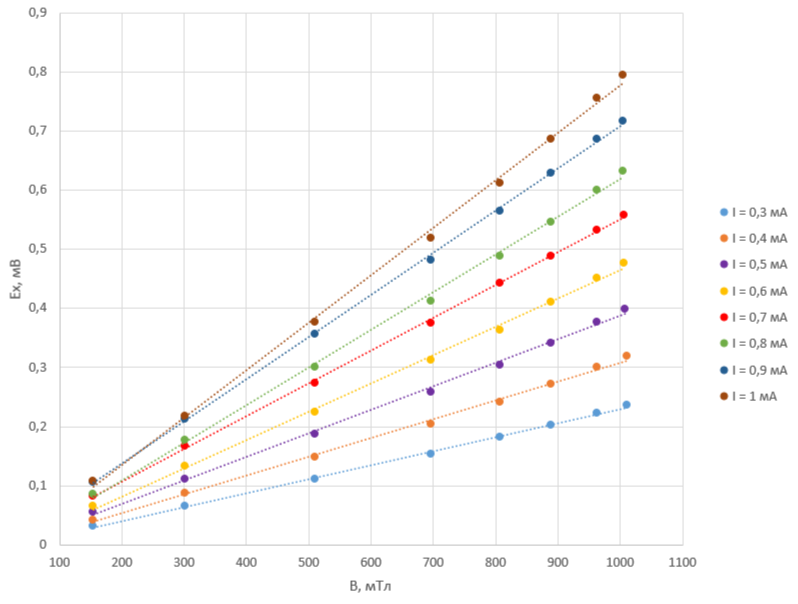
\includegraphics[scale=0.4]{2.png}
    \centering
    \caption*{Графики зависимости $\mathcal{E}_x (B)$.}
\end{figure}

\begin{figure}[h]
\centering
    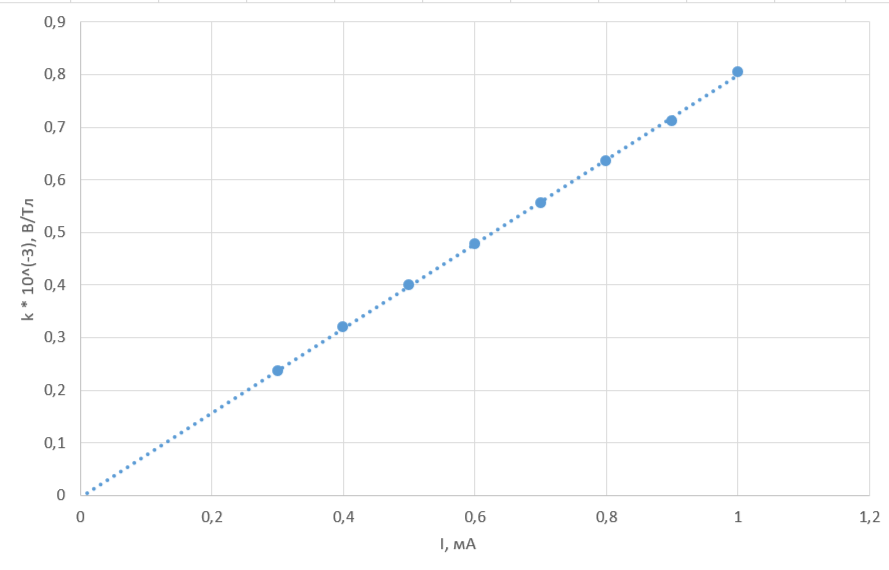
\includegraphics[scale=0.35]{3.png}
    \centering
    \caption*{График зависимости k(I).}
\end{figure}

Апроксимируем полученные данные зависимостью $k = pI$ с помощью МНК:
$$
    p = (797\pm 5)*10^{-3} \dfrac{\text{ В}}{\text{Тл}\cdot\text{А}}
$$
Определим постоянную Холла:
$$
R_H = pa = (797\pm 5)*10^{-6} \dfrac{\text{В}\cdot\text{м}}{\text{Тл}\cdot\text{А}}
$$
Определим концентрацию носителей заряда:
$$
n = \dfrac{1}{R_He} = (784\pm5)\cdot 10^{19} \text{ м}^{-3}
$$

\newpage

\subsection*{3.3. Расчёт удельной проводимости и подвижности}
Hассчитаем удельную проводимость нашего образца. По результатам измерений \\
$ U_{35} = 4,105 $ мВ, $l_{3,5} = 5$ мм; $l = 4$ мм; $I = (1\pm0,01)$ мА. В итоге получаем:
$$
\sigma = \frac{IL_{35}}{U_{35}al} = (304 \pm 3) \text{ } (\text{Ом}\cdot\text{м})^{-1}
$$

Теперь, зная эти характеристики, можно рассчитать подвижность носителей заряда по следующей формуле:

$$
\mu=\frac{\sigma}{en} = 2420 \pm 30 \text{ } \frac{\text{см}^2}{\text{В}\cdot\text{с}}
$$

\section*{4. Вывод}

В ходе выполнения данной лабораторной работы был исследован эффект Холла в полупроводнике, а именно в легированном германии. Была определена постоянная Холла для исследуемого образца $ R_x = (797\pm5) \cdot 10^{-6} \text{ см}^{-3}/\text{Кл} $. Также была вычислена концентрация носителей заряда $ n = (784\pm5) \cdot 10^{19} \text{ м}^{-3}. $

По полярности вольтметра, полярности подключения источника тока и направлению тока в катушках была определён тип проводимости. Тип проводимости оказался электронным.

Также была вычислена подвижность электронов в германии $ \mu = (2420\pm29) \text{ } \text{см}^2/\text{В}\cdot\text{с} $. Однако полученный результат отличается от табличной подвижности электронов в германии $ b_0 = 3900 \text{ } \text{см}^2/\text{В}\cdot\text{с} $. Это может свидетельствовать о наличие примесей исследуемом образце.

Также ощутимый вклад в ошибку полученных данных может внести зависимость характеристик исследуемого образца от температуры, которая могла значительно изменяться в силу прохождения через образец электрического тока.

\end{document}

